% !TeX root = ../main-paper.tex
\section{Experiment 1: NER sensibility to the number of training examples}
\label{sec:ner-xp1}

The constitution of annotated example sets to train a NER model on a target domain is a critical preliminary step.
Often done manually, possibly from bootstrapped annotations, this task is tedious, time-consuming and error-prone.
The ability of a model to perform well even with few training examples is a practical criteria to consider.
In this first experiment, we investigate the performance of the three models when fine-tuned for NER on training sets of decreasing sizes.

\subsection{Dataset}
input: ocr ref (human transcription)
expected output: ner ref (human tagging)

8765 entries, \joseph{FIXME XXXX entities to detect}

\subsection{Metrics}



\subsection{Systems/Variants under test}
We select two deep-learning-based NER models available in packaged software libraries: SpaCy NLP pipelines and CamemBERT.
We also create an additional CamemBERT model pretrained on a collection of unannotated directory entries extracted with Pero-OCR.
The NER layer of each three models is then fine-tuned on historical directories as detailed in \cref{subsection:experiment-1-setup} and \cref{subsection:experiment-2-setup}

\subsubsection{SpaCy}
We use the French pipeline \textit{fr\_core\_news\_lg} provided by SpaCy v.3.2.1\mcite{spacy}, already trained for NER on the deep-sequoia and wikiner-fr corpora.
The default NER labels known to the pipeline are PER, ORG, MISC and LOC.
In experiment 1 the base model is fine-tuned on every of the 8 training sets using the same training parameters.
Early stopping is activated with a patience value of 1600 training steps without improvement of the f1 score.

\subsubsection{CamemBERT pretrained on directories~[CmBERT+ptrn]}
In order to evaluate the benefits of pre-training the language model on OCR texts from domain-related documents, we adapt the CmBERT embeddings using \num{845.000} entries randomly selected wihtin the collection of directories and extracted with Pero-OCR.
We achieve this by training the CmBERT model for 3 epochs on two unsupervised tasks: next sentence prediction and masked language model.


\subsubsection{Huggingface CamemBERT}
\label{sub:ner-xp1-sysytems-huggingcam}
Experiments 1 and 2 rely on the implementation of transformers provided by the software library Huggingface (transformers v.4.15.0, datasets v.1.17.0).
Our baseline CmBERT model is CamemBERT model published on the Hugging Face repository \footnote{\url{https://huggingface.co/Jean-Baptiste/camembert-ner}} and already trained for NER on wikiner-fr.
Its NER head is a linear model with a Softmax function.
CmBERT and CmBERT+ptrn are always fine-tuned using the same parameters, with at most 5000 training steps and an early stopping condition set to 3 evaluations in experiment 1 (5 in experiment 2) without improvement of the f1 score. Evaluations are performed every 100 steps.


\subsection{Protocol}
To do so, we split the gold reference of manually annotated entries into a training set, a development set, and a test set. 
The training set is then gradually reduced in size while maintaining the relative frequency of directories within it.

As the organization and structure of entries varies across directories, the models may learn to overfit on a subset of directories with specific features.
To reduce the evaluation bias, we start by leaving out 3 directories (1690 entries, $\approx 19\%$) from the gold reference to test each model on unseen directories.
Then, a stratified sampling based on the source directory of each entry is run on the remaining set to create a training (6373 entries, $\approx 73\%$ of the gold reference) and a development set (709 entries, $\approx 8\%$).
This sampling procedure is a convenient way to shape both sets, so they reflect the diversity of directories within the gold reference.
The development set is used to evaluate the model performance during the training phase.
To generate smaller training sets, we start from the initial training set and iteratively split it in half using the same stratified sampling strategy as before.
We stop if a directory has only one entry left, or if the current training subset contains less than 30 entries.
Applying this procedure to the initial training set produced 8 training subsets containing 49, 99, 199, 398, 796, 1593, 3186, and 6373 entries.


All tree models are fine-tuned for NER on each training subset.
The performance metrics are measured against the test set after each training.

\subsection{Results and discussion}

Table \ref{tab:experiment-1-models-performances} and Figure \ref{fig:f1-vs-trainsize} show the mean F1 score, precision, and recall computed on the test dataset, for 5 fine tunings of each model and for each of the 8 training subsets.
CmBERT, CmBERT+ptrn and SpaCy NER display the same behaviour: performances increase dramatically with the number of training examples and rapidly reach an area of slower progress around 1000 examples.
The F1 score increases by 4.6 points between 49 and 796 examples for CmBERT (resp. 1.6 for CmBERT+ptrn and 5.1 for SpaCy NER) but only by 1 point between 796 and 6373 examples (resp. 0.6 and 1.4).
The models derived from CamemBERT always outperform the Spacy model.

It appears that pretraining the CamemBERT model on OCRed texts seems worth it only when a the training set used to fine-tune the NER layer is small.
This effect might be due to the differences in nature between the training subsets, whose texts are manually corrected, and the noisy OCR texts used to pretrain CamemBERT.
Indeed, the learned embeddings from the pretraining are specialized on noisy texts and therefore less adapted to clean texts.
The pretraining aims at adapting the model to the vocabulary of the domain and to the errors caused by the OCR, which reveals not helpful and even counter-productive when the texts do not contain these types of errors.


\begin{table}[h!]
\centering
\caption{F1 score, precision and recall measured on the fine-tuned models CmBERT, CmBERT+ptrn and SpaCy NER in experiment 1 for 8 training sets of increasing sizes.}
\begin{tabular}{llrrrrrrrr}
       & Training examples &  49   &  99   &  199  &  398  &  796  &  1593 &  3186 &  6373 \\
       & \% & 0.8   & 1.6   & 3.1   & 6.2   & 12.5  & 25.0  & 50.0  & 100.0 \\
\midrule\bottomrule
\multirow{3}{*}{\rotatebox{90}{F1 score}} & CmBERT &  89.5 &  90.5 &  92.7 &  93.3 &  \textbf{94.1} &  \textbf{94.9} &  \textbf{94.6} &  \textbf{95.1} \\
       & CmBERT-ptrn &  \textbf{92.2} &  \textbf{92.9} &  \textbf{93.6} &  \textbf{93.8} &  93.8 &  94.1 &  \textbf{94.6} &  94.4 \\
       & SpaCy NER &  87.0 &  89.0 &  90.3 &  91.9 &  92.1 &  92.8 &  93.2 &  93.5 \\
\cline{1-10}
\multirow{3}{*}{\rotatebox{90}{Precision}} & CmBERT &  87.4 &  88.7 &  91.5 &  92.7 &  93.3 &  94.9 &  93.9 &  95.1 \\
       & CmBERT-ptrn &  90.8 &  91.8 &  92.9 &  93.0 &  93.0 &  93.4 &  94.1 &  93.9 \\
       & SpaCy NER &  85.6 &  87.7 &  90.0 &  92.0 &  92.4 &  92.8 &  93.1 &  93.7 \\
\cline{1-10}
\multirow{3}{*}{\rotatebox{90}{Recall}} & CmBERT &  91.6 &  92.5 &  93.9 &  93.9 &  94.9 &  94.9 &  95.4 &  95.1 \\
       & CmBERT-ptrn &  93.6 &  94.0 &  94.4 &  94.6 &  94.6 &  94.8 &  95.0 &  94.9 \\
       & SpaCy NER &  88.6 &  90.4 &  90.7 &  91.7 &  91.9 &  92.8 &  93.3 &  93.4 \\
\end{tabular}
\label{tab:experiment-1-models-performances}
\end{table}


\begin{figure}[h!]
	   \center{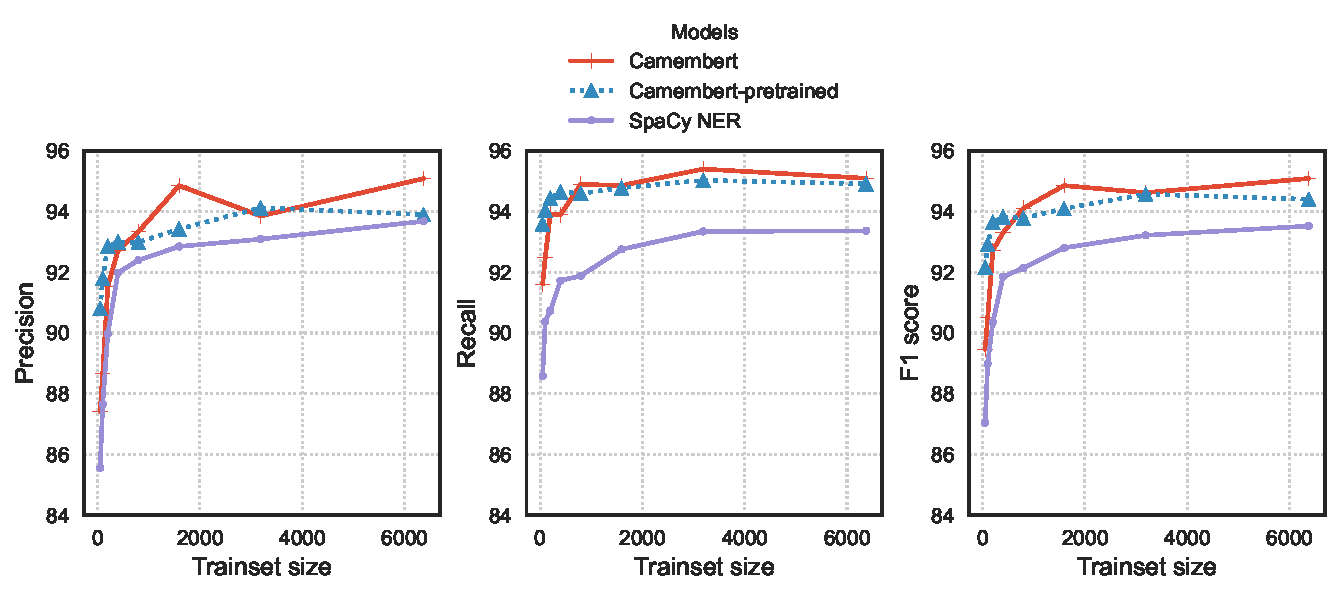
\includegraphics[width=\textwidth]
	       {images/experiment-1-models-performances.pdf}}
	  \caption{\label{fig:f1-vs-trainsize} Precision, recall and f1 score from table~\ref{tab:experiment-1-models-performances}}.
\end{figure}
	                                        

